% Asset ID: A21TrigonometricFunctionsTikZ-003
% Source: Chapter 6 reciprocal graph explanation + CCEA A21-TRIG-LO003
% Related lesson section: Core Theory - Graphs of reciprocal trig functions
% Purpose: Show how y-values of f(x) produce y-values of 1/f(x).

\documentclass[tikz,border=8pt]{standalone}
\usepackage{amsmath}
\usetikzlibrary{positioning, arrows.meta}
\begin{document}
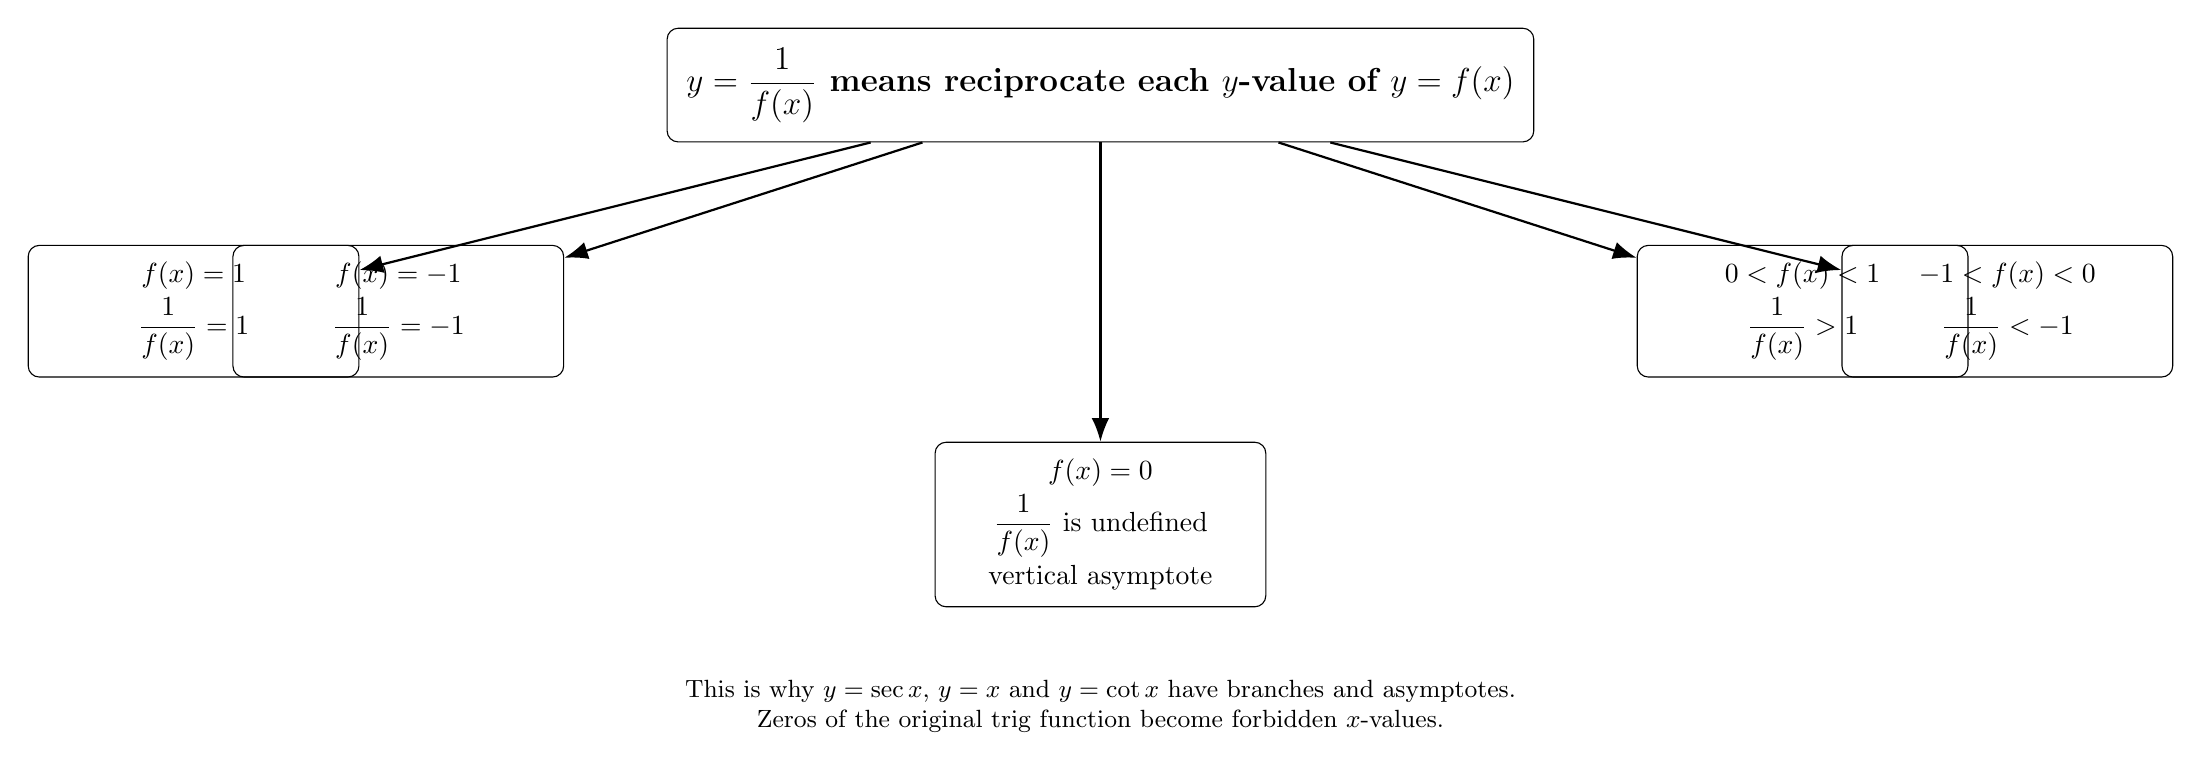
\begin{tikzpicture}[box/.style={draw,rounded corners,align=center,minimum width=4.2cm,minimum height=1.25cm,inner sep=6pt},main/.style={draw,rounded corners,align=center,minimum width=6.5cm,minimum height=1.2cm,inner sep=7pt,font=\large\bfseries},arrow/.style={-{Latex[length=3mm]},thick},note/.style={align=center,font=\small}]
\node[main] (start) at (0,0){$y=\dfrac{1}{f(x)}$ means reciprocate each $y$-value of $y=f(x)$};
\node[box, below left=1.3cm and 3.9cm of start] (one){$f(x)=1$\\[2pt]$\dfrac{1}{f(x)}=1$};
\node[box, below left=1.3cm and 1.3cm of start] (minusone){$f(x)=-1$\\[2pt]$\dfrac{1}{f(x)}=-1$};
\node[box, below right=1.3cm and 1.3cm of start] (smallpos){$0<f(x)<1$\\[2pt]$\dfrac{1}{f(x)}>1$};
\node[box, below right=1.3cm and 3.9cm of start] (smallneg){$-1<f(x)<0$\\[2pt]$\dfrac{1}{f(x)}<-1$};
\node[box, below=3.8cm of start] (zero){$f(x)=0$\\[2pt]$\dfrac{1}{f(x)}$ is undefined\\[2pt]vertical asymptote};
\draw[arrow] (start) -- (one);\draw[arrow] (start) -- (minusone);\draw[arrow] (start) -- (smallpos);\draw[arrow] (start) -- (smallneg);\draw[arrow] (start) -- (zero);
\node[note, below=0.8cm of zero] {This is why $y=\sec x$, $y=\cosec x$ and $y=\cot x$ have branches and asymptotes.\\Zeros of the original trig function become forbidden $x$-values.};
\end{tikzpicture}
\end{document}
